\documentclass[12pt,letterpaper]{article} \usepackage[margin=1in]{geometry}
\usepackage{fancyhdr} \usepackage[utf8]{inputenc} \usepackage{palatino}
\usepackage{microtype} \usepackage{hyperref} \usepackage{graphicx}
\usepackage{lastpage} \usepackage[hang,small,margin=1in]{caption} \usepackage{titlesec}

\renewcommand{\headrulewidth}{0pt} \fancyfoot{} \fancyfoot[C]{\sffamily Page
\thepage\ of \pageref{LastPage}} \pagestyle{fancy}

\titleformat{\section}{\bfseries\MakeUppercase}{\arabic{\thesection}}{1em}{}
\titleformat{\subsection}{\bfseries}{\arabic{\thesection}.\arabic{\thesubsection}}{1em}{}
\titleformat{\subsubsection}{\itshape}{\arabic{\thesection}.\arabic{\thesubsection}.\arabic{\thesubsubsection}}{1em}{}

\setlength{\parindent}{0cm} \setlength{\parskip}{1em}

\captionsetup[figure]{labelfont=it,font=it}
\captionsetup[table]{labelfont={it,sc},font={it,sc}}

\hypersetup{colorlinks, linkcolor = black, citecolor = black, urlcolor
= black} \urlstyle{same}



\begin{document}

\begin{center}
	{\bf\Large Oregon State University \\
		Autonomous Aerial Robotics Team \\
		2013 International Aerial Robotics Competition \\ [1em]
	}
	{\footnotesize Soo-Hyun Yoo, Team Lead, yoos@engr.oregonstate.edu, 740-343-9667 \\
		Ryan Skeele, Ryan McAfee, Kyle Cesare, Zach Reyes, Nathan Brahmstadt, Jordan Crane, Nick Haller \\ [0.5em]
		\emph{204 Rogers Hall, Oregon State University, Corvallis, OR 97333}
	}
\end{center}


\begin{center} \begin{minipage}{5.5in}

\section*{Abstract}

The Oregon State University Aerial Robotics Team will compete in the 2013
International Aerial Robotics Competition with a custom quadrotor capable of
autonomous navigation of a previously unexplored, cluttered indoor environment.
The quadrotor’s chassis and flight system are optimized for reliable 7-minute
flights. A slimmed-down ASUS Xtion Pro Live provides both a depth map and an
RGB video feed of the environment for 3D SLAM and object recognition. A custom
flight control board built around a 32-bit STM32F405 microcontroller allows for
a 1 kHz flight stabilization loop. An array of neodymium magnets on the bottom
of the quadrotor will be used to pick up the USB flash drive.

\end{minipage} \end{center}



\section*{Introduction}

Our primary goal this year is to fully navigate the maze and either simulate
self-destruct when the timer runs out or egress with a complete map of the
space. We will attempt flash drive pickup by identifying the rectangular box
and landing in it with an array of neodynium magnets attached to the bottom of
the quadrotor.

Our 2013 quadrotor was designed with four criteria in mind: lightweight, small,
strong, and simple. The smallest stock carbon tubes, minimalistic aluminum
center brackets, and lightweight 3D printed motor mounts were integrated in
order to meet these criteria.

Two 4S 1000 mAh lithium polymer batteries power the quadrotor’s four Turnigy
D2830-11 brushless DC motors that spin 8x6 3-blade propellers. A 5V switching
regulator further powers a custom flight control board and two onboard
Odroid-X2 mini-PCs clocked at 1.7Ghz. A simple, isolated killswitch mechanism
allows for reliable cutoff of motor power in case of malfunction.

The two Odroids and a custom flight control board built around the STM32F405
32-bit microcontroller provide the necessary computing power to run all
guidance, navigation, and control algorithms onboard the quadrotor itself. An
ASUS Xtion Pro Live stereo camera provides depth and color vision. 

High-level control algorithms on the Odroids run within Robot Operating System
(ROS), which makes it easy to network the two Odroids together to spread the
computing load. RGBDSLAM is used to build up a 3D Octomap of the environment
for SLAM and 2D map extraction.

A custom navigation node using medial axis skeletonization sends flight
commands to the flight control board, which in turn maintains a desired
orientation of the quadrotor with a 1 kHz cascading PID control loop tuned with
the help of a compact test mount designed as an low-friction safety catch to
protect the quad during testing and demonstrations.



\section*{Chassis}

The first decision when custom designing a multi-rotor is how many rotors to
have. A three-rotor design was briefly considered for its smaller number of
motors, but we ultimately decided to continue with a quadrotor since the
additional weight of a tricopter’s servo counteracts any weight savings and
adds a mechanical linkage that may break. In addition, the inherently tilted
steady state of a tricopter while hovering adds unnecessary complexity to
vision and control systems that is not present on a quadrotor.

We optimized our combination of motors and propellers for flight at 1.5 kg.
General consensus among RC enthusiasts on web forums indicate that most
multirotor flight is most efficient if hover throttle duty cycle is around 50\%
of the maximum. We tested motor and propeller combinations and narrowed our
selection down to those capable of providing thrust at this ratio. With
a second and third parameter of size and weight, the resulting motor and
propeller combination is Turnigy D2830/11 1000kV outrunners with master
airscrew 8x6 3-blade propellers. This combination provides a maximum thrust of
over 750g per motor.

Lightweight, small, strong, and simple were the four most important
requirements set before designing the frame. The arms of the quadrotor uses the
smallest carbon tubes that could be guaranteed straight by the manufacturer.
The arms are attached in an X formation wrapped in the center with
a carbon-aramid weave. Two aluminum rings act as a clamp to provide
a supporting moment on each arm as well as a mounting plate for the
electronics.

Motor mounts designed as plugs to the carbon tubes were optimized for weight
and strength using finite element analysis (FEA, see
Figures~\ref{fig:feastress} and \ref{fig:feastrain}). The motor mount design is
capable of accepting any motors up to 40mm in diameter. The design allows for
multiple orientations of the motor and propellor, with the chosen configuration
(Figure~\ref{fig:mmf}) used to minimize torque on the carbon tubes. With the
first configuration (Figure~\ref{fig:mmi}) the torque caused significant
vibration issues.  The current configuration decreases vibrations by minimizing
the moment arm of the propellers to the motor mounts. 

\begin{figure}[!h]
	\centering
	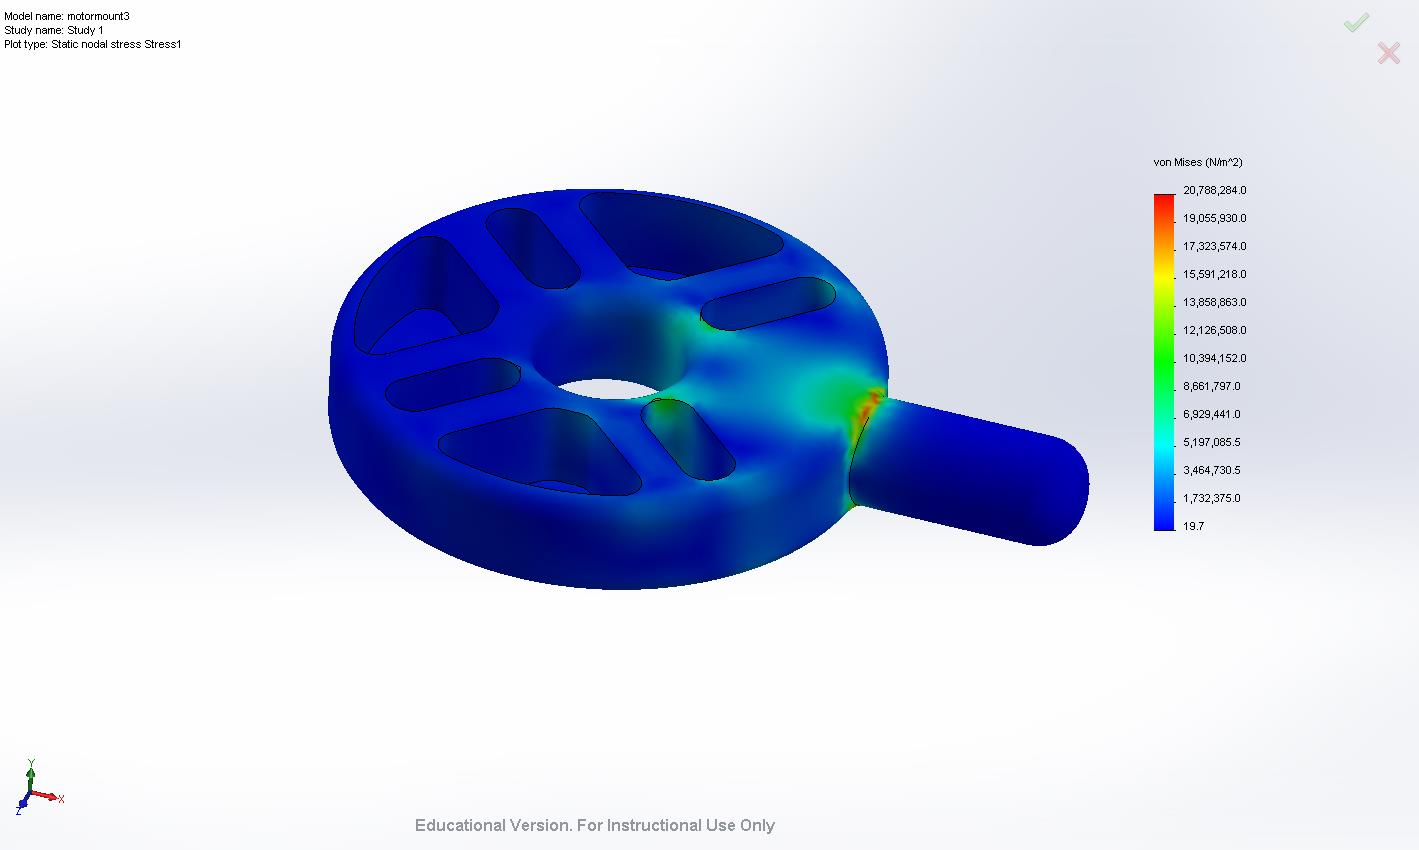
\includegraphics[width=0.6\textwidth]{img/fea_stress.jpg}
	\caption{FEA with red indicating high levels of stress. Forces applied perpendicular to flat mount.}
	\label{fig:feastress}
\end{figure}
 
\begin{figure}[!h]
	\centering
	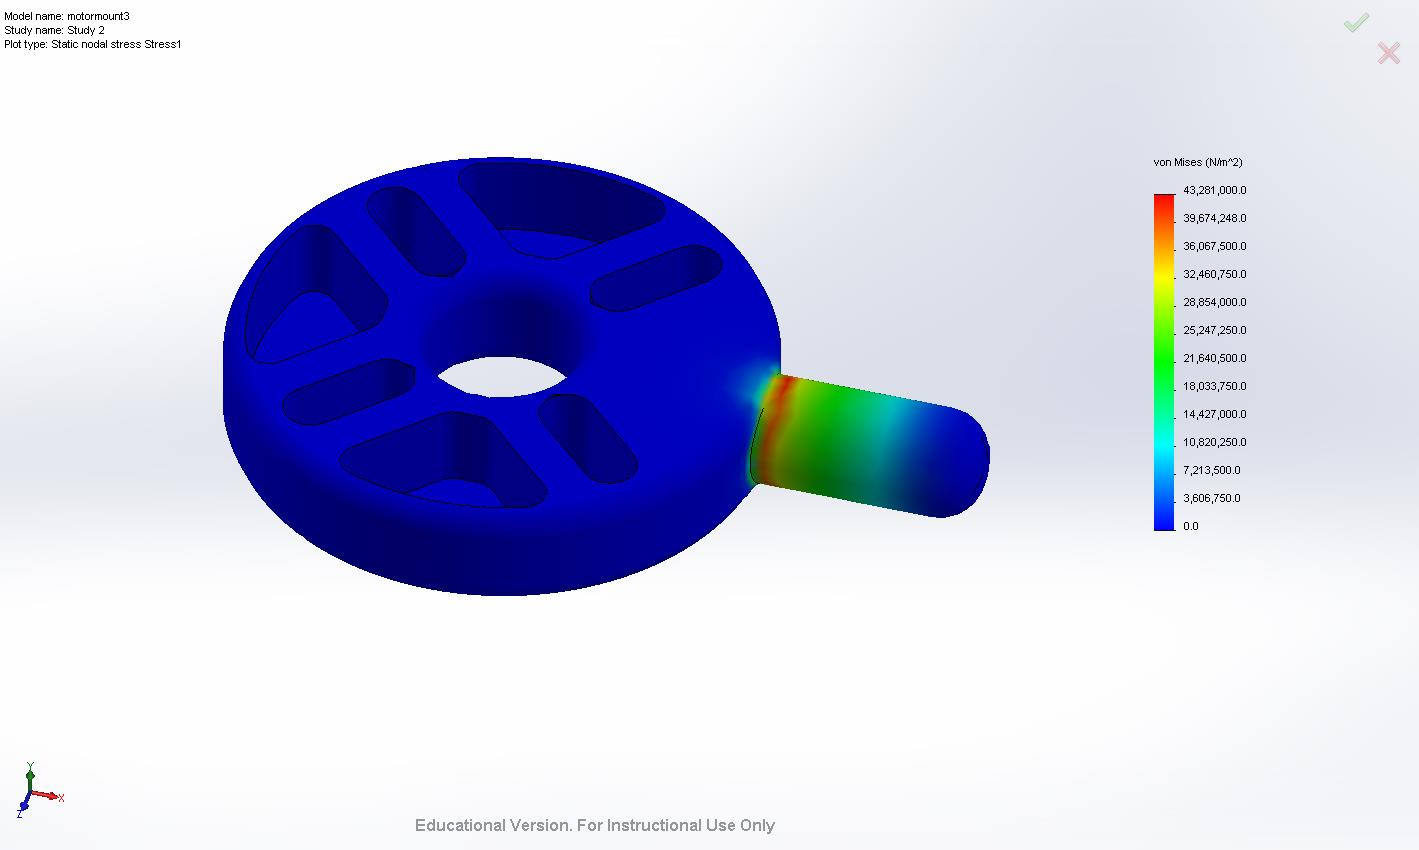
\includegraphics[width=0.6\textwidth]{img/fea_strain.jpg}
	\caption{FEA with red indicating high levels of stress. Forces applied torsionally simulating torques from figure 4.}
	\label{fig:feastrain}
\end{figure}

\begin{figure}[!h]
	\centering
	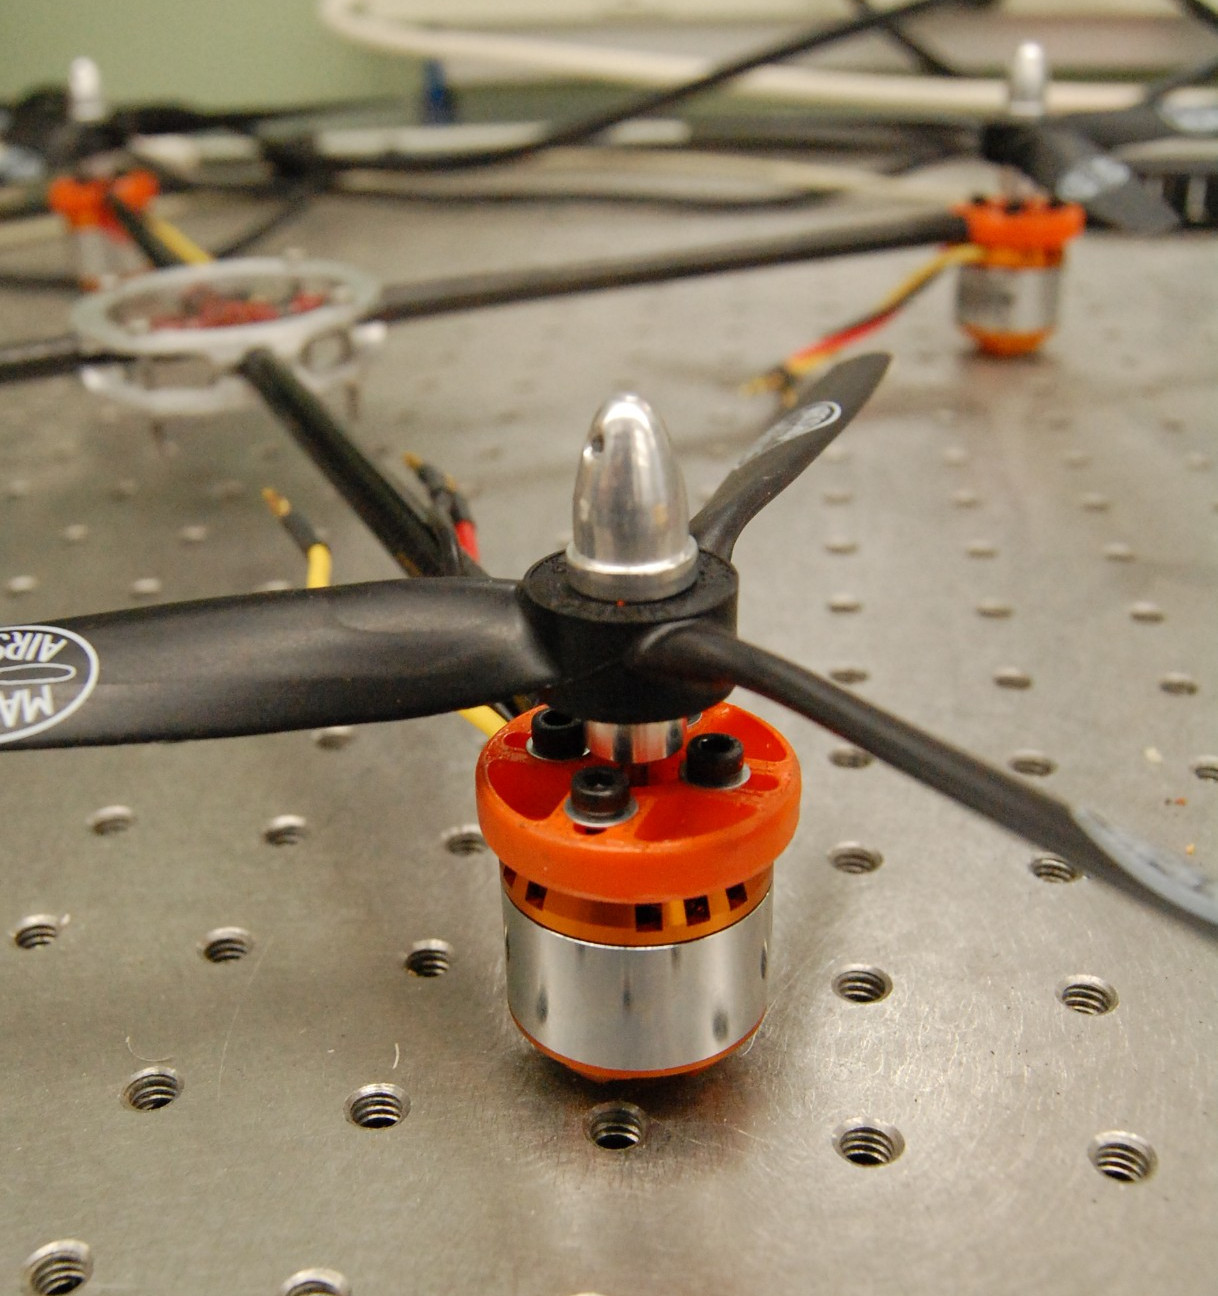
\includegraphics[width=0.5\textwidth]{img/motor_mount_final.jpg}
	\caption{Final motor mount configuration. Having the two rotating masses on either side of the mount reduces vibration.}
	\label{fig:mmf}
\end{figure}

\begin{figure}[!h]
	\centering
	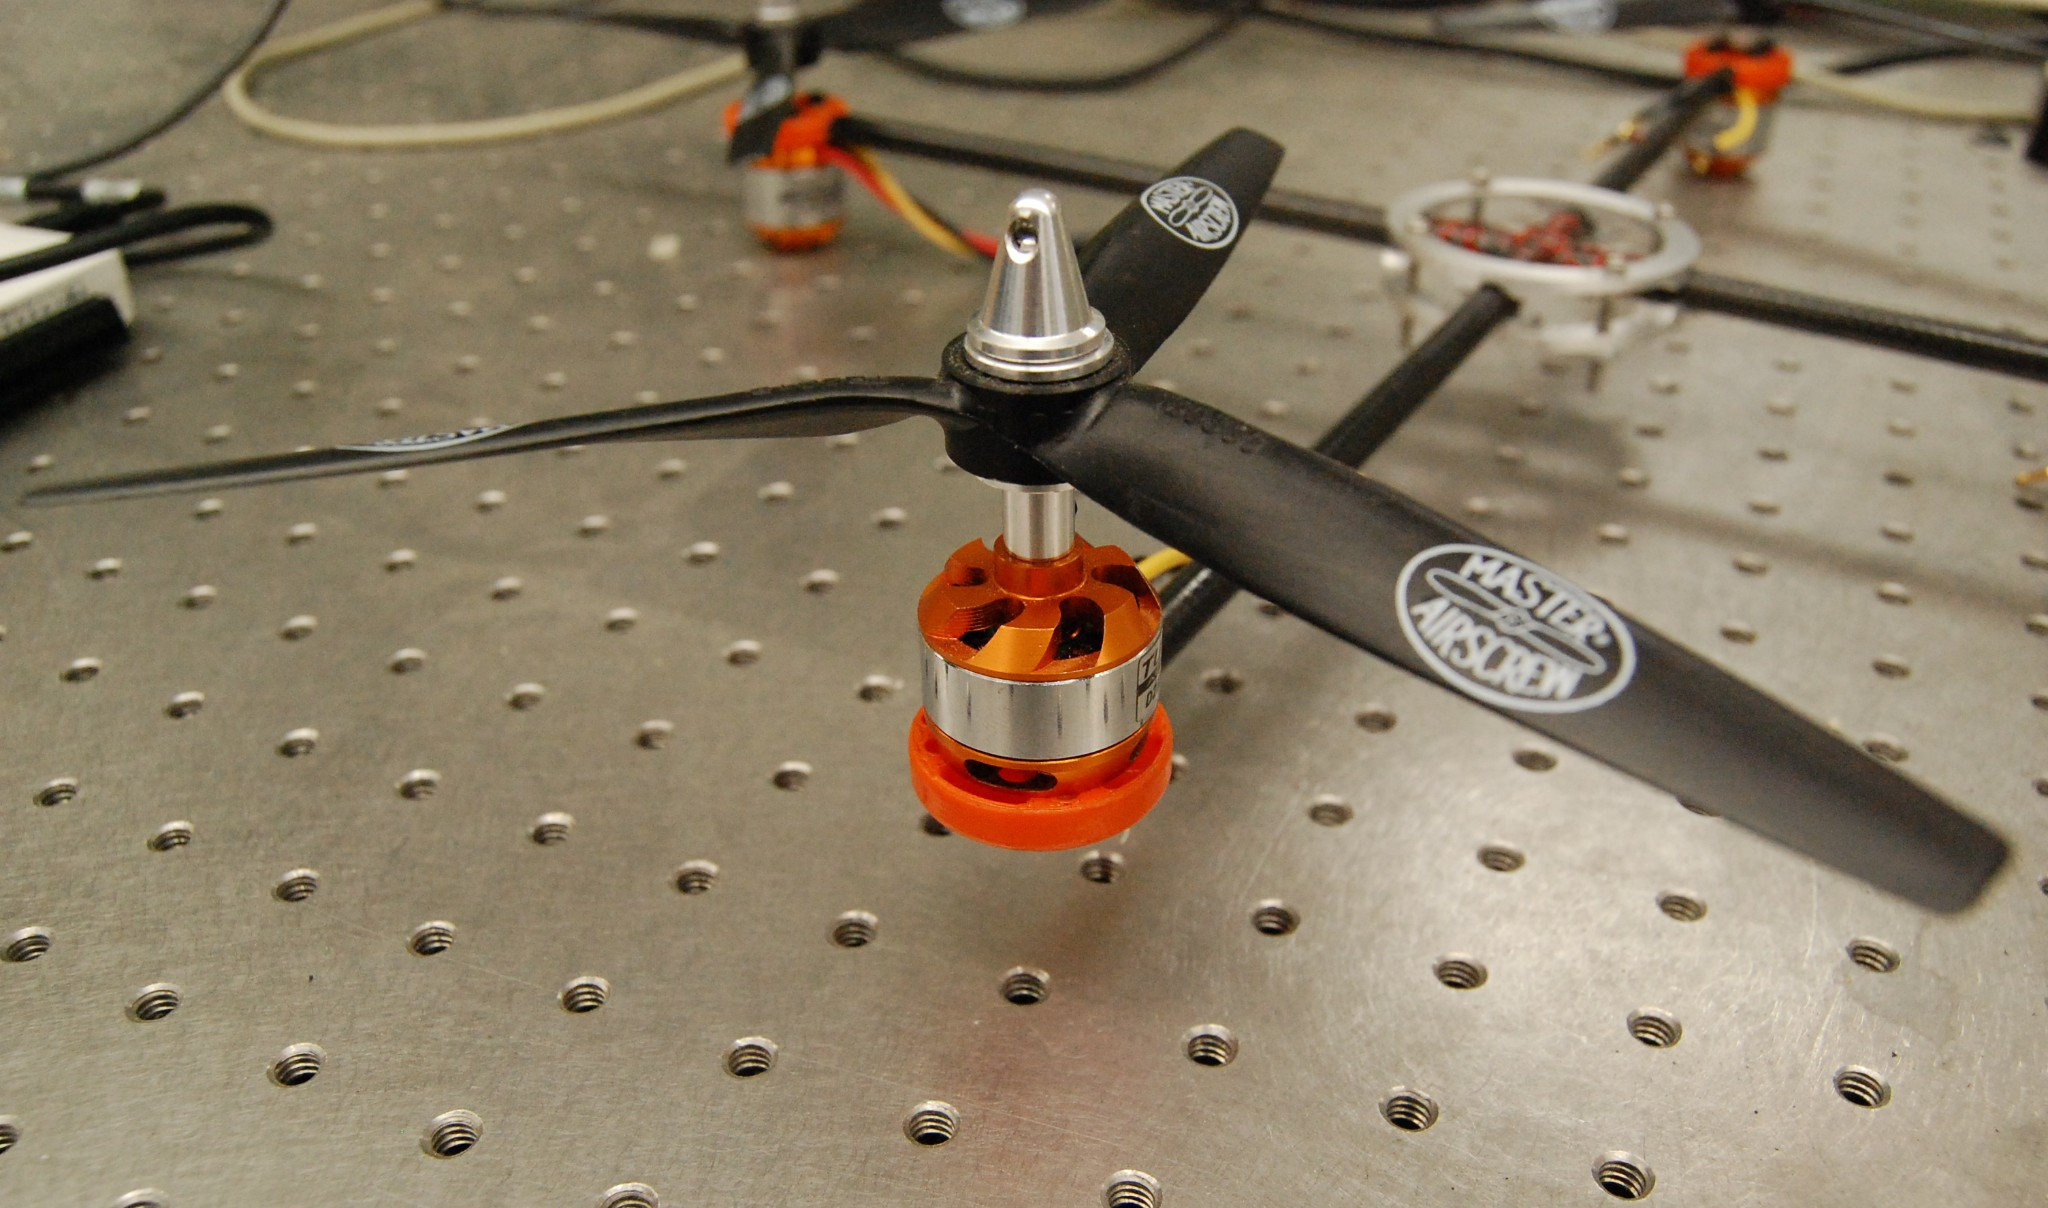
\includegraphics[width=0.6\textwidth]{img/motor_mount_initial.jpg}
	\caption{Initial motor mount configuration. The longer moment arm made the mount prone to vibrations.}
	\label{fig:mmi}
\end{figure}



\section*{Electronics}

\subsection*{Power}

All electronics on the quadrotor are powered by two 4S 1000 mAh lithium polymer
batteries wired in parallel. While using a single 2000 mAh battery would have
been ideal, we were unable to find such a battery with the desired dimensions.

Four Turnigy D2830-11 1000kv brushless motors powered by Turnigy Plush 18A ESCs
turning 8x6 Master Airscrew 3-blade propellers provide us with our performance
characteristic of 50\% throttle hover.

The Texas Instruments PTN78020WAH wide-input voltage-adjustable switching
regulator provides steady 5V power at up to 6A for onboard logic and small
actuators. The regulator is integrated into our flight control board and also
powers a linear regulator that in turn supplies 3.3V to the logic bus.


\subsection*{Onboard Computing: Odroid-X2}

In 2012, many teams, including our own, were wracked by wireless interference
due to overusage of the 2.4 GHz band in the competition arena. We decided to
work around this issue by confining all computation to the quadrotor itself,
with only a 900 MHz downlink for killswitch activation.

The Odroid-X2 is a 4”-square mini-PC built around the Samsung Exynos 4412
quad-core ARM Cortex-A9 clocked at 1.7 GHz (Figure~\ref{fig:odroids}). Each
quadrotor is built with two Odroids onboard, networked via Ethernet for sharing
computational load. At full load, each Odroid can draw up to 2A at 5V.

\begin{figure}[!h]
	\centering
	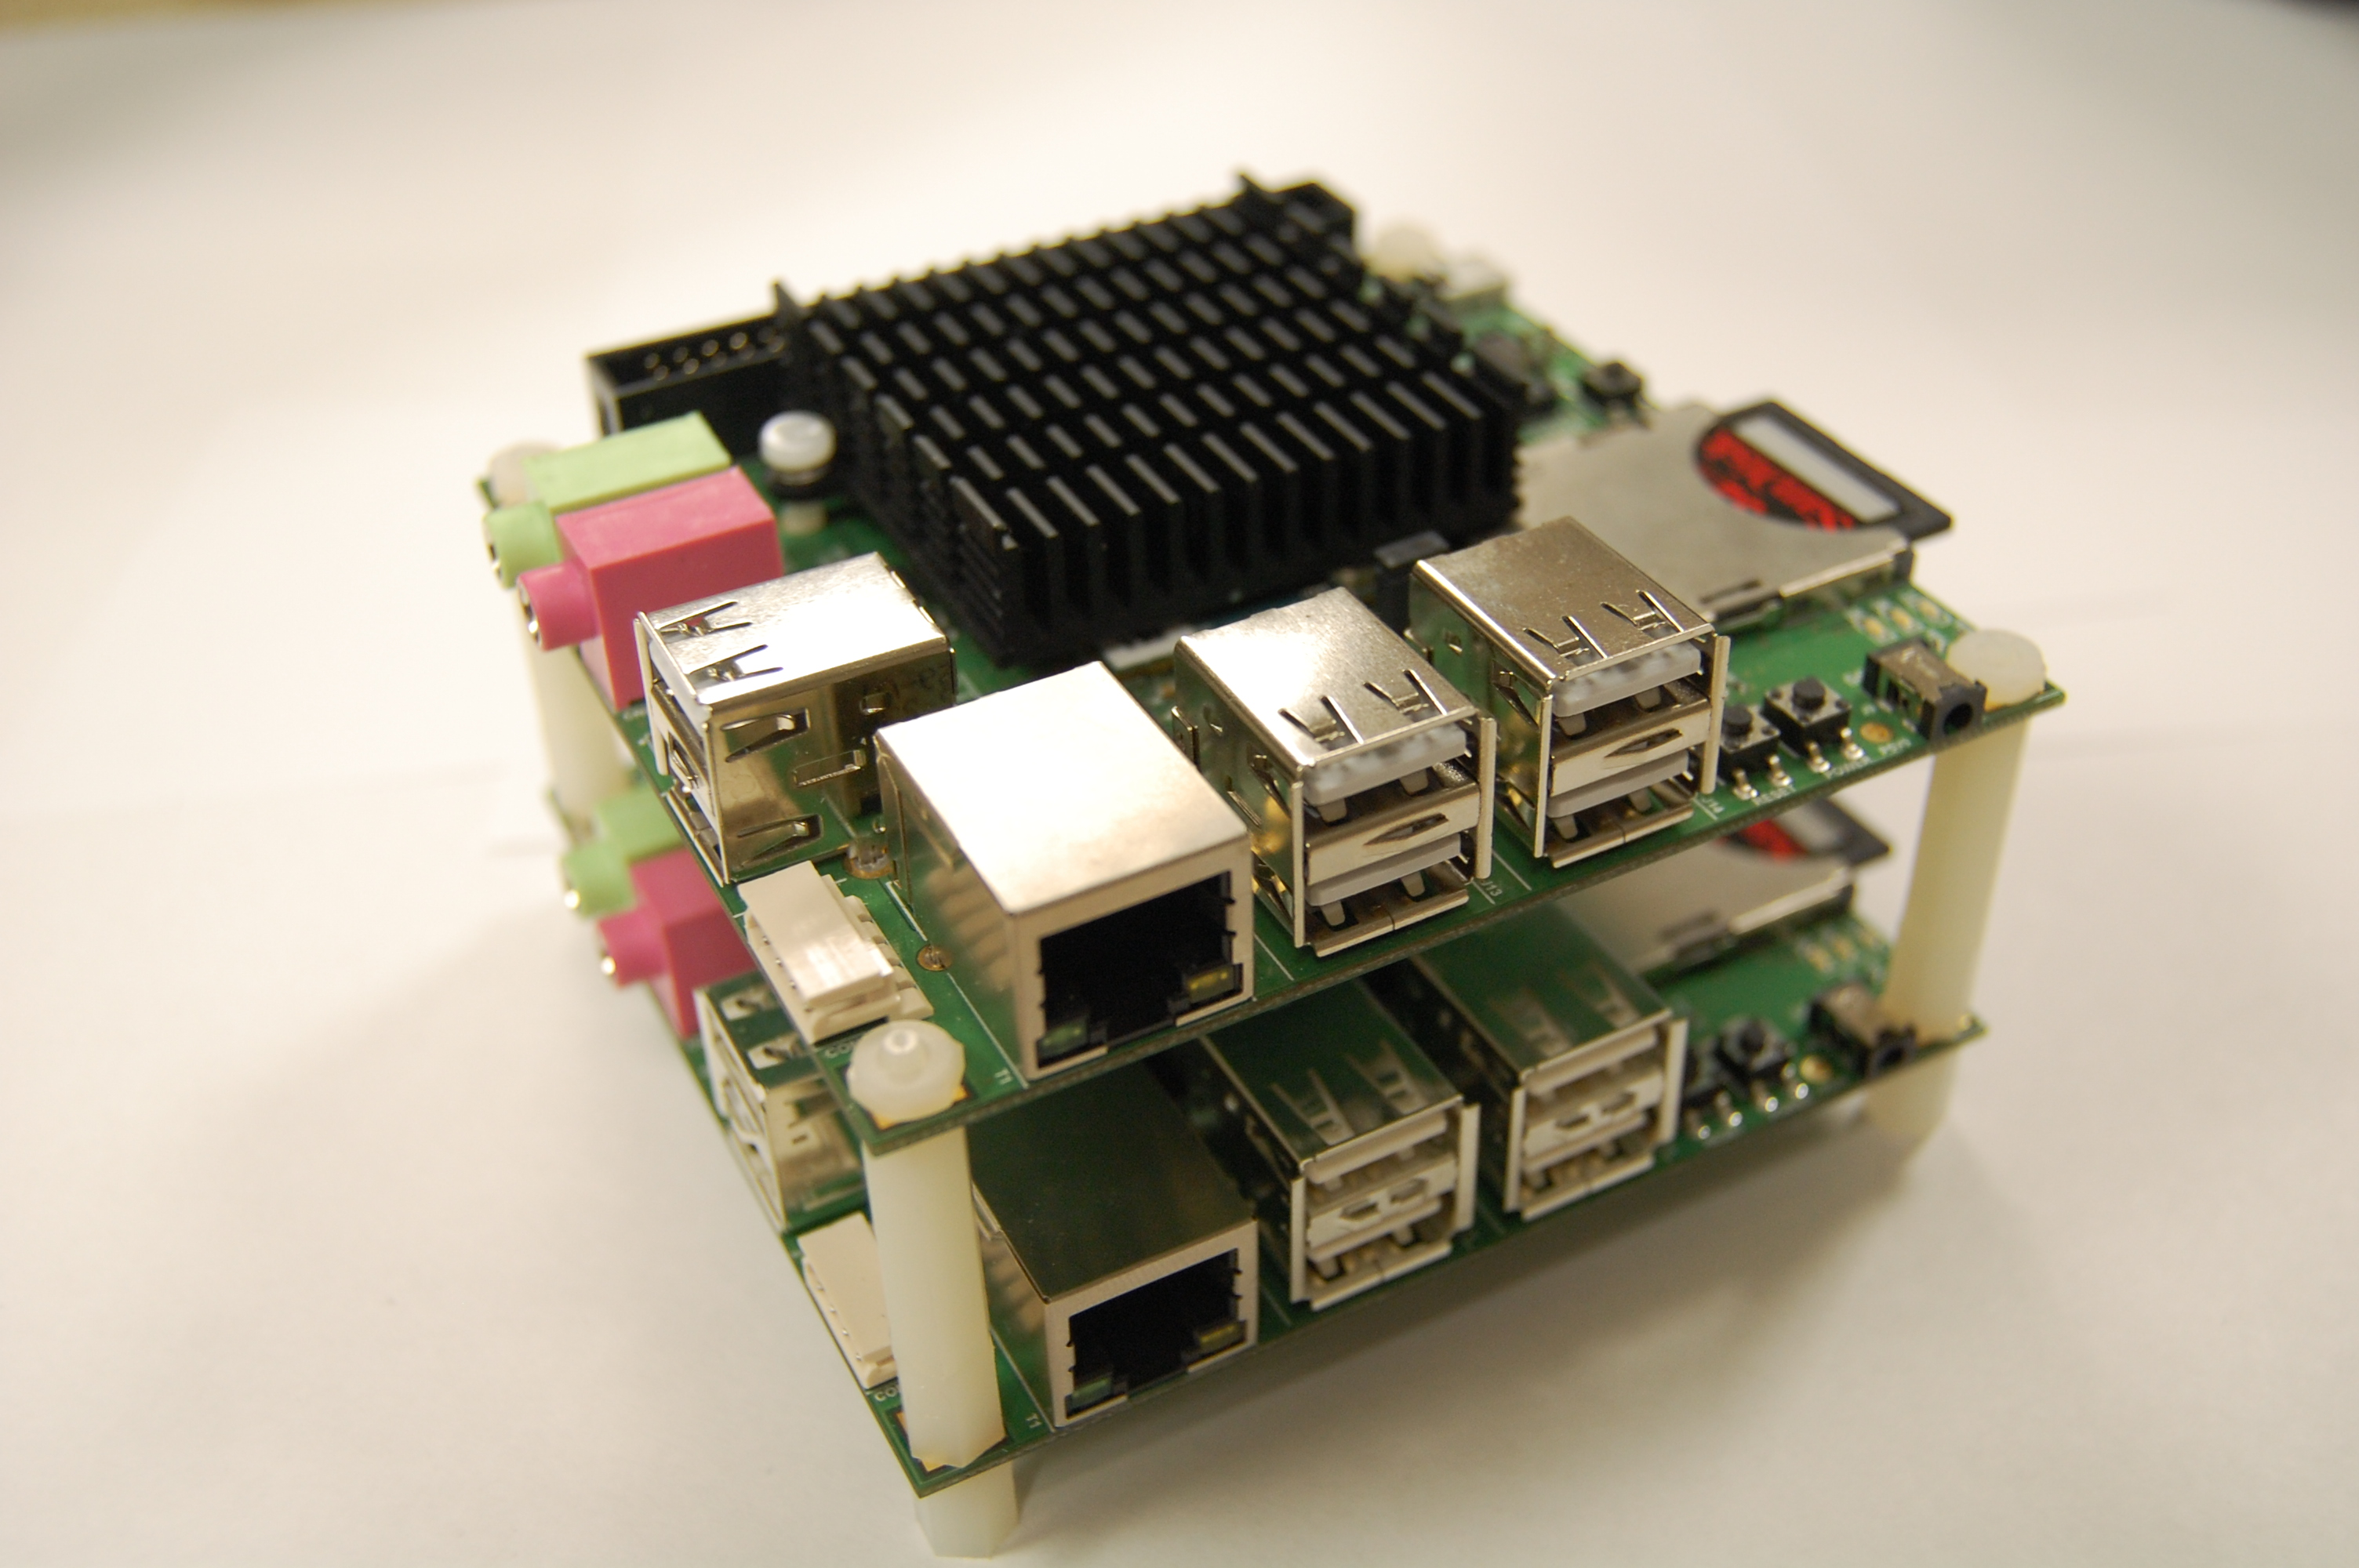
\includegraphics[width=0.6\textwidth]{img/odroid_stack.jpg}
	\caption{Stack of two Odroids.}
	\label{fig:odroids}
\end{figure}


\subsection*{Vision: ASUS Xtion Pro Live}

The Xtion Pro Live (Figure~\ref{fig:xtion}) is much like the more commonly
known Microsoft Kinect in that it outputs a 30 Hz depth map and a 1280x720 RGB
video stream (up from the 640x480 video of the Kinect). Unlike the Kinect,
however, the Xtion Pro is physically slimmer and lighter and lacks the Kinect’s
heavy motorized base, making it well-suited for use on small, lightweight UAVs.
It uses the same PrimeSense chip for generating the depth maps, so it functions
identically to the Kinect where software is concerned.

\begin{figure}[!h]
	\centering
	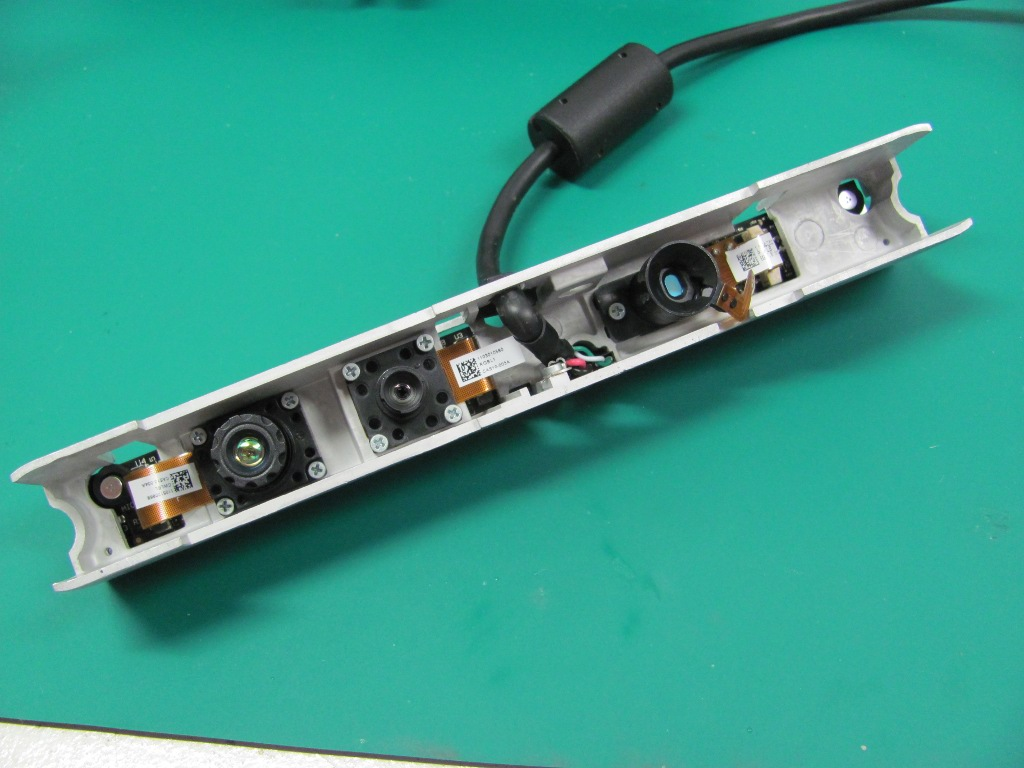
\includegraphics[width=0.6\textwidth]{img/xtion.jpg}
	\caption{ASUS Xtion Pro Live without external housing.}
	\label{fig:xtion}
\end{figure}

The depth map from the Xtion Pro is fed to a SLAM process on one of the Odroids
onboard the quadrotor and is the sole sensor providing positional awareness for
the quadrotor.


\subsection*{Flight Control Board (STM32F405)}

The 2012 flight control board built around the ATXmega128a3, while sufficient
for basic flight, was scrapped in favor of using the much more powerful
STM32F405 in order to achieve 1 kHz flight stabilization. Although we do not
yet take full advantage of this higher control loop frequency, it effects lower
gyroscopic drift and allows for higher PID gains and tighter control.

The flight control board controls four ESCs with 400 Hz PWM signals and has
four SPI connectors available for future use of a custom 1 kHz-capable,
SPI-enabled ESC. The flight control board receives flight commands from either:

\begin{itemize}
	\item The Odroids over a 460800 baud USART bus for autonomous control, or
	\item The XBee over a 38400 baud USART bus for manual control.
\end{itemize}

Orientation estimates are calculated using feedback from an InvenSense MPU-6000
six-axis gyroscope/accelerometer chip, which is polled at 1 kHz in sync with
the flight control loop.


\subsection*{Killswitch and Wireless Communication}

The killswitch provided by the IARC was modified to operate at 16.8V (4S
lithium polymer) and is wired in series between the battery and ESCs. The PWM
signal required to keep the killswitch closed is generated by a 900 MHz XBee
Pro and is not associated at all with the flight control board.

The onboard XBee is paired with another XBee held by a human operator. A pair
of pins between the two XBees are configured to mirror each other such that the
pin on the handheld XBee can be given a PWM signal (generated by
a microcontroller, also a part of the handheld device) and mirrored by the
onboard XBee. This minimizes the amount of software and electronics involved,
thereby maximizing reliability.

Although the XBee link to the killswitch is currently the only form of wireless
communication we plan to employ during competition, we will attempt to stream
video from the quadrotor to the base station via 5 GHz wifi. If this is
successful, we will once again try offboard guidance and navigation as
appropriate.



\section*{Software}

RGBDSLAM on the onboard computers builds up a 3D Octomap using the Xtion Pro.
A 2D map is extracted from this 3D model with arbitrary precision. A navigation
process then uses the 2D map to generate a desired flight path and sends
appropriate flight commands to the embedded flight control board. The flight
control board then maintains the quadrotor at the desired orientation with
a 1 kHz control loop.


\subsection*{Robot Operating System}

Robot Operating System (ROS) is a collection of libraries and tools that allows
developers from around the world to contribute software packages such as device
drivers, messaging libraries, and visualizers in a consistent format for others
to use.

We have developed our high-level control systems to operate within this
software architecture. This allows us to use third-party joystick drivers,
point cloud libraries, and SLAM algorithms, which frees us from having to
reimplement solved problems.

In addition, due to ROS’s exclusive use of TCP/UDP network protocols for
inter-process communication, ROS nodes on the two separate Odroids can
communicate with each other with no additional software, save for basic network
configuration.


\subsection*{RGBDSLAM and Octomap}

Traditionally, point clouds, elevation maps, and multi-level surface maps have
been used to represent a map generated using SLAM. However, the sheer volume of
data involved in keeping track of the physical world can overwhelm even the
fastest desktop computers available today.

One way in which to represent 3D environments is to use a grid of
uniformly-sized cubes (voxels). However, the grid must be initialized in memory
prior to exploration, which makes this method memory-intensive and limits
exploration to the space within the preallocated grid.

Octomap is a novel approach to storing and manipulating 3D information that has
been designed to meet the following three requirements:

\begin{itemize}
	\item Probabilistic representation: measurements are, by nature, uncertain.
		The model must reflect this uncertainty.
	\item Modeling of unmapped areas: the robot has to be able to avoid
		traversing unmapped areas before measuring said areas.
	\item Efficiency: since the map is a central point in the system, it must
		be efficient with regards to access times and memory consumption.
\end{itemize}

3D space can be represented hierarchically using octrees, which recursively
divide each voxel into eight subvoxels. Due to this hierarchical nature, an
octree can easily be cut at any level to obtain a downsampled map of the
environment.

The Octomap library was made freely available as a ROS package by Hornung and
his group. We use RGBDSLAM’s implementation of the Octomap library on the two
Odroids onboard the quadrotor and hope to achieve near-realtime performance
despite limited computational resources.


\subsection*{2D Map Extraction}

It is trivial to either extract a 2D slice from the 3D Octomap by specifying
a Z-height or to project all points to a plane by ignoring the Z-height. This
2D slice is then published to the navigation node as an image.


\subsection*{Navigation}

First, the 2D extracted map is skeletonized via a medial axis morphological
transformation, which generates a set of points equidistant from at least two
points on the object’s boundary. This gives us a very rough idea of valid paths
we can follow (Figure~\ref{fig:medial_axis}). We then filter these points be
their distances from obstacles.

\begin{figure}[!h]
	\centering
	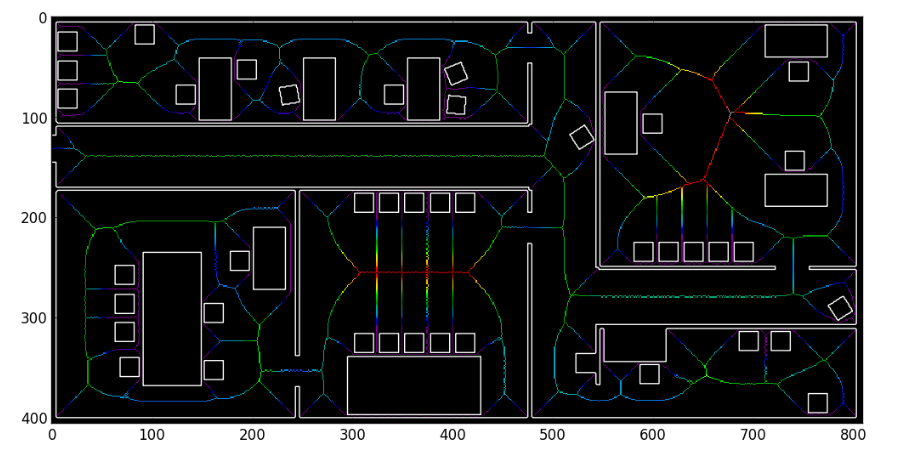
\includegraphics[width=0.6\textwidth]{img/medial_axis.png}
	\caption{Skeletonized 2D map.}
	\label{fig:medial_axis}
\end{figure}

Next, we find all path endpoints (Figure~\ref{fig:identify_endpoints}). This is
accomplished by a computing a template matrix cross-correlation, where the
templates are line segment endings in each of the eight directions.

\begin{figure}[!h]
	\centering
	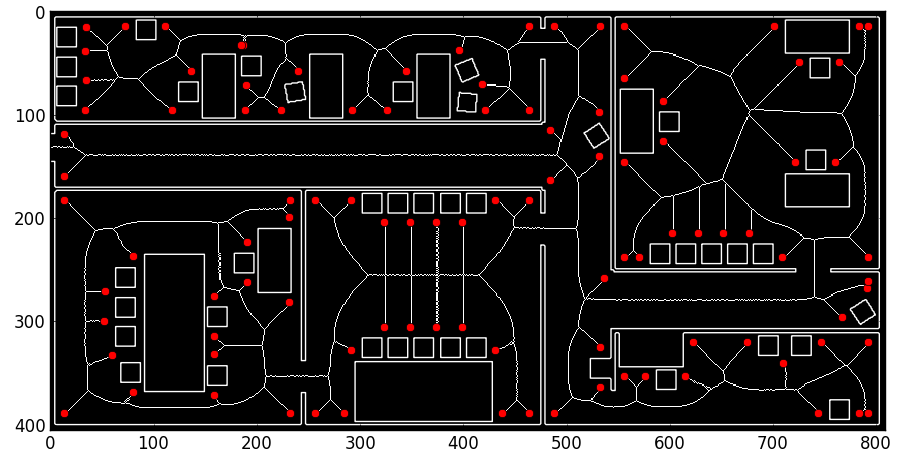
\includegraphics[width=0.6\textwidth]{img/identify_endpoints.png}
	\caption{Endpoints of skeleton identified.}
	\label{fig:identify_endpoints}
\end{figure}

We can then use the combination of the skeletonization and the endpoints to
generate paths to each endpoint, given any starting location on the map
(Figure~\ref{fig:generate_paths}).

\begin{figure}[!h]
	\centering
	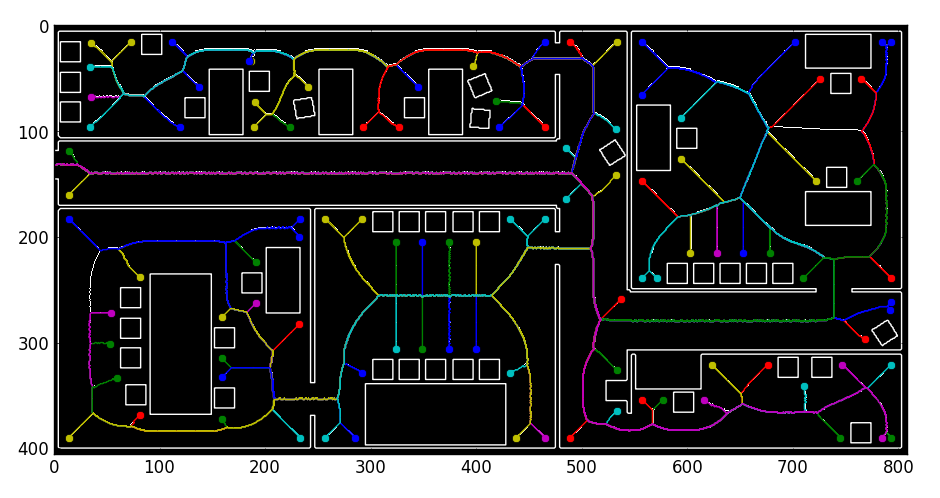
\includegraphics[width=0.6\textwidth]{img/generate_paths.png}
	\caption{Paths to endpoints generated.}
	\label{fig:generate_paths}
\end{figure}

Once we have these paths, the navigation node commands the flight controller
with a desired orientation that will cause the quadrotor to move. We always
choose the nearest (via path geometric cost) unvisited endpoint. Following this
algorithm, and updating the skeletonization as we explore previously unknown
areas, we should be able to traverse the entire map and eventually find the USB
flash drive.

The above is accomplished using a combination of Python, numpy, scipy, and
scikit-image.


\subsection*{Flight Control}

In order to mitigate the added complexity of the STM32F4 over the ATXmega128
used on our 2012 quadrotor, we write our controllers as processes within
ChibiOS, a real-time operating system for embedded devices. ChibiOS provides
basic functionality for managing threads, mutexes, and a hardware abstraction
layer. We run two main threads: a 1 kHz flight control loop and a 100 Hz
communications loop. Since these threads are created in the same generic format
such as the following control loop thread, we can easily add more processes:

\begin{center} \begin{minipage}{5.5in}

{\scriptsize

\begin{verbatim}
/*
 * Control loop
 */
static WORKING_AREA(wa_control_thread, 128);
static msg_t control_thread(void *arg)
{
    (void) arg;
    chRegSetThreadName("control");

    systime_t time = chTimeNow();

    /* DCM of body in global frame. */
    float dcm_bg[3][3];
    m_init_identity(dcm_bg);

    /* Motor duty cycles */
    float motor_dc[4];

    while (TRUE) {
        time += MS2ST(CONTROL_DT*1000);   // Next deadline in 1 ms.

        update_ahrs(CONTROL_DT, dcm_bg);
        run_controller(dcm_bg, motor_dc);
        update_motors(motor_dc);

        palTogglePad(GPIOA, 6);

        chThdSleepUntil(time);
    }

    return 0;
}
\end{verbatim}

}

\end{minipage} \end{center}

The 1 kHz control loop stabilizes the quadrotor in the air by doing the
following in succession:

\begin{enumerate}
	\item Read IMU (gyroscope and accelerometer)
	\item Update orientation estimate
	\item Run cascading PID controllers on current and desired orientations
	\item Update ESC duty cycles appropriately
\end{enumerate}

This code was largely ported over from code used in our 2012 tricopter (built
experimentally, not used for competition). The higher loop frequency lends
improved stability and reduced gyroscopic drift, thus making higher-speed
maneuvers feasible.



\section*{Testing and Safety}

\subsection*{Table Mount}

A restrictive three-dimensional arm was built to safely test and demonstrate
the quadrotor (Figure~\ref{fig:quad_test_mount}). The arm limits the
quadrotor’s ability to move. This was developed in response to previous crash
tests that resulted in hours of wasted time fixing broken hardware.

\begin{figure}[!h]
	\centering
	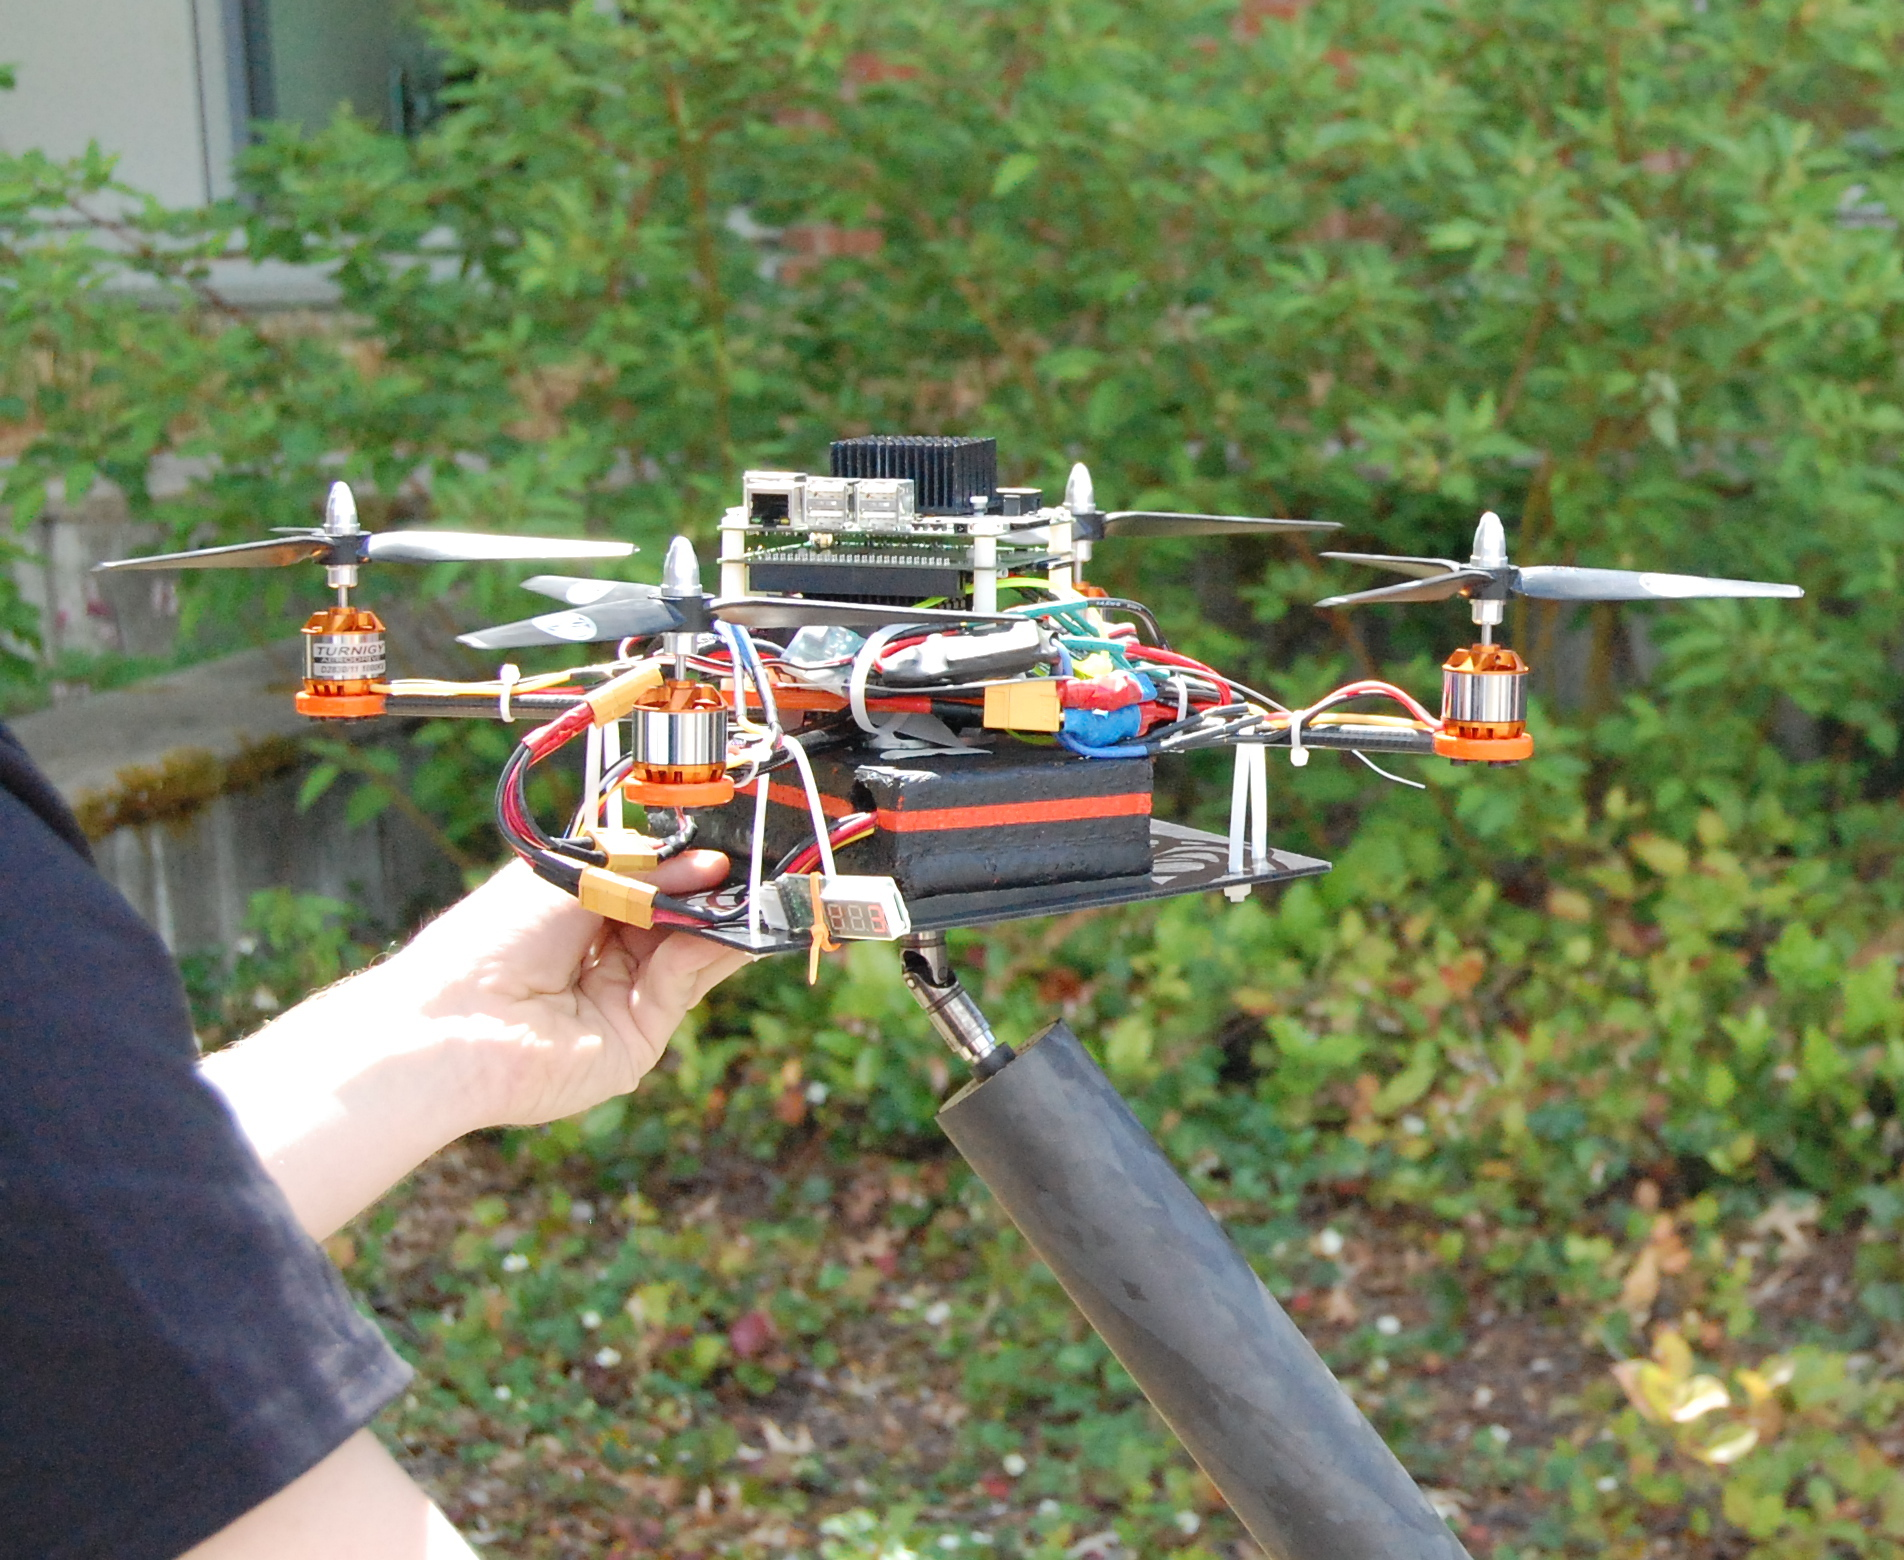
\includegraphics[width=0.6\textwidth]{img/quad_test_mount.jpg}
	\caption{Quadrotor on test mount.}
	\label{fig:quad_test_mount}
\end{figure}

Several design solutions were explored culminating in the current telescoping
arm design. One such alternative was a C-shape frame structure, with a pulley
system that was able to move the quadrotor horizontally and vertically. This
idea was impractical because it was large, which would have been too unwieldy
to be used portably for public demos.

Our final design is capable of being collapsed when not in use and extended
during testing. The arm, when clamped to a table, is able to rotate 360 degrees
and provides the quadrotor with a freedom of motion 4 feet in diameter and
2 feet in height. The test stand allows us to reduce risk of catastrophic
damage to our quadrotor during testing.



\section*{Conclusion}

The OSU Autonomous Aerial Robotics Team has constructed an ambitious entry to
the Mission 6 challenge. With custom flight control breakout board, onboard
processing for vision and navigation, and a lightweight chassis for longer
flight time, the quadrotor is a completely autonomous and untethered flying
machine.

Porting over flight control software to the real time operating system ChibiOS
allowed us to take advantage of the ARM processor and its capability to
multithread.

Optimizing the chassis to meet competition requirements gave us new challenges.
We applied root cause failure analysis to determine vibrations were caused by
long moment arms from the propellers. In addition we developed a way to safely
perform full flight tests without fear of damaging the quadrotor.

Developing a solution to radio interference problems introduced the hurdle of
onboard processing. Processing power was perhaps the biggest challenge of this
year and has led to much of the software design choices.

Success at the 2013 competition will come with fully autonomous mapping of the
building and shutdown or egress at the end of flight time.

Next year’s team looks to advance this years progress with the exploration of
a more elaborate sensor/vision system.



\section*{Thank You}

We would like to thank the OSU College of Engineering, the Oregon NASA Space
Grant Consortium, DW Fritz Automation, and the National Science Foundation for
their generous support.

The OSU Aerial Robotics Team is supported in part through NASA/Oregon Space
Grant Consortium, grant NNX10AK68H.

\end{document}
